\chapter{Les modules}

	\marginicon{objectif}
	Dans ce chapitre, nous voyons pourquoi et comment découper un algorithme
	en modules (morceaux d'algorithmes).

\section{Introduction}

	Outre le choix de noms de variables explicites et une indentation
	correcte, tout bon programmeur se doit de veiller à la clarté et la
	lisibilité de ses algorithmes. Si ces qualités sont relativement aisées
	à assurer dans les premiers exemples et exercices abordés, il n’en est
	pas de même lorsque croissent la complexité et la longueur des
	algorithmes. Il est courant que les lignes de codes de programmes se
	comptent en centaines ou en milliers. Dès lors, le découpage en modules
	est indispensable. En outre, lors de l’écriture d’un algorithme sur
	papier, on conseille dans un souci de lisibilité qu’aucun des modules
	ne dépasse la longueur d’une page.
	
	Illustrons l’approche modulaire sur l’exercice du chapitre précédent
	demandant de calculer le maximum de 3 nombres. Commençons par écrire la
	solution du problème plus simple : le maximum de 2 nombres.

	\cadre{
	\begin{pseudo}
	\Module{max2}{}{}
		\Decl a,b,max : réels
		\Read a,b
		\If{a > b}
			\Let max \Gets a
		\Else
			\Let max \Gets b
		\EndIf
		\Write max
	\EndModule
	\end{pseudo}
	}
	
	Pour le maximum de 3 nombres, il existe plusieurs approches. Voyons
	celle-ci :

	\cadre{
	\begin{pseudo}
		\Stmt Calculer le maximum des deux premiers nombres, soit temp
		\Stmt Calculer le maximum de temp et du troisième nombre, ce qui donne le résultat.
	\end{pseudo}
	}

	{Sur base de cette idée, comment faire à présent
	pour introduire le calcul du maximum de 2 nombres dans l’algorithme
	calculant le maximum de 3 nombres ? Une solution consiste à
	«~copier-coller~» les lignes de code du module
	}\textstyleCodeInsr{{max2}}{
	dans le module
	}\textstyleCodeInsr{{max3}}{,
	toutefois en adaptant son contenu au contexte de ce module : les
	nombres
	}\textstyleCodeInsr{{a}}{
	et
	}\textstyleCodeInsr{{b}}{
	ne doivent plus être systématiquement lus et la valeur du maximum ne
	doit plus être systématiquement affichée. Ainsi
	}\textstyleCodeInsr{{temp}}{
	est calculé et ré-utilisé dans un calcul ultérieur. Ceci donnerait :}

	\cadre{
	\begin{pseudo}
	\Module{max3}{}{}
		\Decl a,b,c,temp,max : réels
		\Read a,b,c
		\If{a > b}
			\Let temp \Gets a
		\Else
			\Let temp \Gets b
		\EndIf
		\If{temp > c}
			\Let max \Gets temp
		\Else
			\Let max \Gets c
		\EndIf
		\Write max
	\EndModule
	\end{pseudo}
	}

	Bien que correcte, cette démarche est cependant déconseillée et peut
	s’avérer fastidieuse, spécialement dans le cas de «~grands~»
	algorithmes. Imaginons qu’il aurait fallu de cette façon «~mixer~» deux
	algorithmes d’une cinquantaine de lignes chacun. Le résultat serait un
	algorithme d’une centaine de lignes qui perdrait en lisibilité et
	clarté. De plus, l’opération effectuée n’est pas sans risques : que se
	passerait-il si les deux modules contiennent chacun une variable nommée
	de manière identique ? Cette «~transplantation~» demande donc la
	vérification de toutes les variables utilisées, la réécriture des
	lignes de déclarations de variables de façon à y inclure celles du
	module «~greffé~», le «~raccord~» correct des données lues et écrites
	par ce module aux variables du module principal, etc… 
	
	Imaginons, par exemple, que l'on doit calculer le
	maximum de 4 ou même 5 nombres. Le résultat serait un code long et
	composé de lignes fort proches. Une erreur serait vite arrivée et
	serait difficile à détecter.
	
	L’idéal serait de pouvoir garder deux modules séparés, conservant chacun
	leur spécificité (l’un calculant le maximum de deux nombres et l’autre
	le maximum de trois nombres) mais de leur permettre de communiquer
	entre eux pour s’échanger des données ou des résultats de calculs. Nous
	allons voir deux solutions.

\section{Passage de paramètres}

	Pour pouvoir faire communiquer les modules entre eux, il faut les
	équiper d’une «~interface~» de transmission des variables appelée
	l’\textbf{en-tête }du module et qui contient une déclaration de
	variables qu’on appellera ici \textbf{paramètres} du module. 
	
	Les variables accompagnées d’une flèche vers le bas (\textsf{↓}) sont
	des \textbf{paramètres d’entrée} qui reçoivent des données au
	\textbf{début} de l’exécution du module (données qui ne doivent donc
	plus être lues) tandis que celles accompagnées d’une flèche vers le
	haut (\textsf{↑}) sont des \textbf{paramètres de sortie} qui permettent
	de renvoyer des résultats à l’\textbf{issue} de l’exécution du module
	(résultats qui ne doivent donc plus être écrits). 

	Par exemple, ceci donnerait pour le module \textstyleCodeInsr{max2} :

	\cadre{
	\begin{pseudo}
	\Module{max2}{a\In, b\In : réels, max\Out : réel}{}
		\If{a > b}
			\Let max \Gets a
		\Else
			\Let max \Gets b
		\EndIf
	\EndModule
	\end{pseudo}
	}

	Notons que, sous cette forme, ce module est devenu «~inactif~», il ne
	lit rien ni n’écrit rien, mais il est cependant prêt à être utilisé. Il
	suffit pour cela de lui fournir les valeurs de \textstyleCodeInsr{a} et
	\textstyleCodeInsr{b} (paramètres d’entrée) pour qu’il entre en action.
	Une fois le maximum calculé, celui-ci est affecté à la variable
	\textstyleCodeInsr{max} qui – en tant que paramètre de sortie –
	contiendra et renverra le résultat voulu.

	{Pour faire appel aux services de ce module, il
	suffit à présent d’écrire son nom suivi d’un nombre de variables (ou
	d'expressions) en accord avec son entête. Montrons par
	un exemple comment le module
	}\textstyleCodeInsr{{max3}}{
	peut faire appel au module
	}\textstyleCodeInsr{{max2}}{:}

	\cadre{
	\begin{pseudo}
	\Module{max3}{}{}
		\Decl a,b,c,temp,max : réels
		\Read a,b,c
		\Stmt max2( a, b, temp )
		\Stmt max2( temp, c, max )
		\Write max
	\EndModule
	\end{pseudo}
	}

	{
	{L’instruction
	}\textstyleCodeInsr{{max2(a, b,
	temp)}}{ se déroule comme suit :}}
	
	\begin{liste}
	\item {
	{le contenu des variables
	}\textstyleCodeInsr{{a}}{
	et
	}\textstyleCodeInsr{{b}}{
	est affecté aux paramètres d’entrée
	}\textstyleCodeInsr{{a}}{
	et
	}\textstyleCodeInsr{{b}}{
	du module
	}\textstyleCodeInsr{{max2}}{,
	puis ce module peut entrer en action ;}}
	\item {
	{à l’issue du module
	}\textstyleCodeInsr{{max2}}{,
	la valeur du paramètre de sortie
	}\textstyleCodeInsr{{max}}{
	est communiquée à la variable
	}\textstyleCodeInsr{{temp}}{,
	qui contient à présent le maximum de
	}\textstyleCodeInsr{{a}}{
	et
	}\textstyleCodeInsr{{b}}{.}}
	\end{liste}

	{
	{L’instruction
	}\textstyleCodeInsr{{max2(temp, c,
	max)}}{ se déroule comme suit :}}
	
	\begin{liste}
	\item {
	{le contenu des variables
	}\textstyleCodeInsr{{temp}}{
	et
	}\textstyleCodeInsr{{c}}{
	est affecté aux paramètres d’entrée
	}\textstyleCodeInsr{{a}}{
	et
	}\textstyleCodeInsr{{b}}{
	du module
	}\textstyleCodeInsr{{max2}}{,
	puis ce module peut entrer en action ;}}
	\item {
	{à l’issue du module
	}\textstyleCodeInsr{{max2}}{,
	la valeur du paramètre de sortie
	}\textstyleCodeInsr{{max}}{
	est communiquée à la variable
	}\textstyleCodeInsr{{max}}{,
	qui contient à présent le maximum des 3 nombres de départ.}}
	\end{liste}

	{Il est évident que la présence de ces deux
	instructions dans le module
	}\textstyleCodeInsr{{max3}}{
	implique la présence du module
	}\textstyleCodeInsr{{max2}}{
	«~aux alentours~» du premier, c’est-à-dire que ces deux modules doivent
	se trouver sur le même support d’écriture de
	l'algorithme complet.}

	{
	{Implicitement, on a introduit ici un nouveau
	type de primitive, l’}{\textbf{appel à un
	}}{\textbf{module}}{\textit{
	}}{qui consiste en la simple écriture de son
	nom dans le code. Cette }{instruction est
	reconnue comme telle car elle ne s’apparente pas aux autres types
	}{d’instruction vus précédemment (primitives
	}\textstyleMotCl{{lire}}{,
	}\textstyleMotCl{{écrire}}{,
	affectation
	(}\Gets{)}{,
	structures }{de contrôle
	}\textstyleMotCl{{si}}{,
	}\textstyleMotCl{{selon
	que}}{,
	}\textstyleMotCl{{tant
	que}}{,
	}\textstyleMotCl{{pour}}{,
	etc.) Lorsque l’ordinateur rencontre cette instruction, il va
	rechercher si un module portant ce nom existe. Une fois ce module
	trouvé, les paramètres }{\textit{ad
	hoc}}{ lui sont communiqués et toutes les
	instructions le composant sont exécutées séquentiellement. Arrivé à
	l’issue du module, les paramètres de sortie sont communiqués au module
	appelant et le déroulement de celui-ci se poursuit là où il avait été
	interrompu.}}

	{\bfseries Remarques}

	\begin{liste}
	\item {
	{un paramètre peut être à la fois paramètre
	d’entrée et de sortie ; on le fait suivre alors de la double flèche
	}{↓↑}{ ;}}
	\item {
	si tous les paramètres sont en entrée, on peut omettre les flèches;}
	\item {
	la présence de ces paramètres n’est pas obligatoire, on peut envisager
	un module sans paramètre de sortie (par ex. un module qui reçoit en
	entrée un nombre et dont la seule fonction est de l’afficher à
	l’écran), ou inversement sans paramètre d’entrée (un module qui simule
	un lancer de dé, et renvoie en paramètre une valeur aléatoire entre 1
	et 6) ;}
	\item {
	{pour appeler correctement un module, il faut
	fournir des noms de variables, des expressions ou des constantes
	}{\textbf{en même
	nombre}}{ et en même ordre que les paramètres
	du module ;}}
	\item {
	en outre, les types des variables doivent correspondre entre l’appel et
	l’en-tête du module ;}
	\item {
	ne peut être affectée à un paramètre d’entrée du module qu’une
	constante, une expression ou une variable préalablement affectée ;}
	\item {
	à un paramètre de sortie d’un module doit toujours correspondre une
	autre variable, jamais une constante ou une expression ;}
	\item {
	il faut s’assurer qu’à l’issue du module, tous les paramètres de sortie
	aient été affectés lors de l’exécution de ce module.}
	\end{liste}

\section{Variables locales}

	Dans le cadre de ce cours d’algorithmique,
	nous n’envisagerons que l’utilisation de 
	\textbf{variables locales}. 
	Toute variable est \textbf{locale} au module 
	dans lequel elle apparait, ce qui veut dire que son existence
	est ignorée en dehors de ce module. 
	Nous n’envisageons donc pas ici l’utilisation de 
	\textbf{variables globales} 
	(variables dont le contenu est reconnu 
	par tous les modules d’un programme).

	Précisons qu'une variable locale est aussi
	\textbf{dynamique}, c’est-à-dire qu’un emplacement en mémoire lui est
	réservé durant l’exécution du module où elle est déclarée. Une fois
	l’exécution terminée, cet emplacement est récupéré en mémoire.

	Plutôt qu’une restriction, cette propriété est
	une aide confortable au programmeur : si, de
	façon fortuite, des variables appartenant à des modules différents
	possédaient le même nom, il n’y aurait pas d’interférence entre ces
	variables, ni confusion possible de leur
	contenu. Par exemple, dans le module
	\textstyleCodeInsr{max2}, les paramètres d’entrée 
	\textstyleCodeInsr{a}, \textstyleCodeInsr{b}
	ainsi que le paramètre de sortie \textstyleCodeInsr{max}
	sont locaux à ce module. 
	Ce serait aussi le cas de toute autre variable temporaire 
	déclarée dans le module.

	Notons au passage que les variables déclarées dans l’entête du module ne
	doivent plus l’être dans la partie «~déclaration de variables~» de ce
	module. Mais toutes les variables utilisées dans un module doivent être
	déclarées, soit dans son entête, soit dans sa déclaration. Le
	non-respect de cette règle provoquerait une erreur d’exécution.

	Pour illustrer le fonctionnement des variables
	locales, voici encore une nouvelle version de l’algorithme incluant une
	fonctionnalité qui va empêcher l’utilisateur d’entrer des nombres
	strictement négatifs. Le module
	\textstyleCodeInsr{lirePositif} ci-dessous
	vérifie si un nombre lu est positif et affiche un message
	d'erreur sinon. Le texte complet de l’algorithme est
	le suivant :

	\cadre{
	\begin{pseudo}
	\Module{max3}{}{}
		\Decl a,b,c,temp,max : réels
		\Stmt lirePositif(a)
		\Stmt lirePositif(b)
		\Stmt lirePositif(c)
		\Stmt max2( a, b, temp )
		\Stmt max2( temp, c, max )
		\Write max
	\EndModule
	\end{pseudo}
	}

	\cadre{
	\begin{pseudo}
	\Module{lirePositif}{a\Out : réel}{}
		\Read a
		\If{a<0}
			\Error Le nombre n'est pas positif !
		\EndIf
	\EndModule
	\end{pseudo}
	}

	\cadre{
	\begin{pseudo}
	\Module{max2}{a\In, b\In : réels, max\Out : réel}{}
		\If{a > b}
			\Let max \Gets a
		\Else
			\Let max \Gets b
		\EndIf
	\EndModule
	\end{pseudo}
	}

	Dans cet exemple, les trois modules en jeu utilisent 
	une variable nommée \textstyleCodeInsr{a}; 
	il n’y a cependant aucune confusion possible. 
	Ainsi, à l’issue du deuxième appel du module
	\textstyleCodeInsr{lirePositif}, 
	le contenu de son paramètre \textstyleCodeInsr{a}
	est affecté à la variable \textstyleCodeInsr{b}
	du module \textstyleCodeInsr{max2}.

\section{Module renvoyant une valeur}

	Un deuxième type de module est le 
	\textbf{module renvoyant une valeur}. 
	(On désigne aussi ce type de modules par le terme \textbf{fonction}).
	Son entête est du type suivant :

	\cadre{
	\begin{pseudo}
	\ModuleSign{exemple}{var1\In:type1,var2\In:type2,\dots,varN\In:typeN}{typeRes}
	\end{pseudo}
	}

	Il se distingue du module précédemment étudié par la flèche de renvoi à
	droite, et possède les particularités suivantes :

	\begin{liste}
	\item {
		{ce module renvoie
		}{\textbf{une}}{
		}{\textbf{valeur}}{
		}{\textbf{qui n’est pas affectée à une variable
		de
		}}{\textbf{sortie~}}{;}}
	\item {
		{à droite de la flèche de renvoi ne se trouve
		donc pas le nom d’un paramètre de sortie, mais le
		}{\textbf{type}}{ de la
		valeur renvoyée ;}}
	\item {
		\textstyleCodeInsr{{typeRes}}{
		est le type de la valeur renvoyée ; en théorie, ce peut être un type
		simple (entier, réel, booléen, chaine, caractère), un type structuré ou
		même un tableau (ces types seront vus dans les chapitres suivants). En
		pratique il conviendra de s’en tenir aux limitations du langage utilisé
		;}}
	\item {
		\textstyleCodeInsr{{var1}}{,
		...,
		}\textstyleCodeInsr{{varN}}{
		sont les paramètres du module (aussi appelés
		}{\textbf{arguments}}{)
		; ce sont le plus souvent des paramètres d’entrée, les paramètres de
		sortie }{étant plus rares dans ce type de
		module ;}}
	\item {
		ces arguments deviennent automatiquement des variables locales du module
		; déclarées dans son en-tête, elles ne doivent plus l’être dans la
		partie déclarative ;}
	\item {
		{la valeur renvoyée est définie à la fin du
		module via la primitive
		}\textstyleCodeInsr{{retourner}}{
		}\textstyleCodeInsr{{résultat}}{,
		où
		}\textstyleCodeInsr{{résultat}}{
		est une variable (ou plus généralement une expression) de type
		}\textstyleCodeInsr{{typeRes}}{
		;}}
	\item {
		pour appeler ce type de module, on utilise son nom \textbf{comme celui
		d’une variable} dans le module appelant, mais jamais à gauche du signe
		d’affectation.}
	\end{liste}

	Comme précédemment, il faut veiller, lors de l’appel du module renvoyant
	une valeur, à ce que le nombre d’arguments ainsi que leur type
	correspondent à ceux spécifiés dans l’entête.

	Pour exemple, transformons une fois de plus la
	dernière version de notre algorithme.
	Plutôt que de renvoyer un résultat via un paramètre de sortie, 
	les modules \textstyleCodeInsr{lirePositif} et
	\textstyleCodeInsr{max2} renvoient à présent 
	chacun uniquement une valeur de type \textit{réel}.
	Noter que le premier de ces modules n’a pas d’argument.
	Noter également la façon d’appeler ces deux modules.

	\cadre{
	\begin{pseudo}
	\Module{max3}{}{}
		\Decl a,b,c,temp,max : réels
		\Let a \Gets lirePositif()
		\Let b \Gets lirePositif()
		\Let c \Gets lirePositif()
		\Let temp \Gets max2(a,b)
		\Let max  \Gets max2(temp,c)
		\Write max
	\EndModule
	\end{pseudo}
	}

	\cadre{
	\begin{pseudo}
	\Module{lirePositif}{}{réel}
		\Decl a : réel
		\Read a
		\If{a<0}
			\Error Le nombre n'est pas positif !
		\EndIf
		\Return a
	\EndModule
	\end{pseudo}
	}

	\cadre{
	\begin{pseudo}
	\Module{max2}{a\In, b\In : réels}{réel}
		\Decl max : réel
		\If{a > b}
			\Let max \Gets a
		\Else
			\Let max \Gets b
		\EndIf
		\Return max
	\EndModule
	\end{pseudo}
	}

	L'écriture avec une valeur de retour permet une
	écriture plus compacte :

	\cadre{
	\begin{pseudo}
	\Module{max3}{}{}
		\Decl a,b,c,temp,max : réels
		\Let a \Gets lirePositif()
		\Let b \Gets lirePositif()
		\Let c \Gets lirePositif()
		\Let max  \Gets max2(max2(a,b),c)
		\Write max
	\EndModule
	\end{pseudo}
	}

	ou encore (mais on perd un peu en clarté) :

	\cadre{
	\begin{pseudo}
	\Module{max3}{}{}
		\Decl a,b,c,temp,max : réels
		\Let a \Gets lirePositif()
		\Let b \Gets lirePositif()
		\Let c \Gets lirePositif()
		\Write max2(max2(a,b),c)
	\EndModule
	\end{pseudo}
	}

	ou même (et là, ce n'est plus du tout lisible !) :

	\cadre{
	\begin{pseudo}
	\Module{max3}{}{}
		\Write max2(max2(lirePositif(),lirePositif()),lirePositif())
	\EndModule
	\end{pseudo}
	}

\section{Un exemple complet}

Synthétisons les notions vues dans ce chapitre au travers
d'un exemple complet.

\marginicon{exercice}
\begin{Emphase}{Exercice résolu : Écart entre 2 moments}
	Étant donné deux moments dans une journée donnés chacun par trois
	nombres (heure, minute, seconde), écrire un algorithme qui calcule et
	affiche le délai écoulé entre ces deux moments en heure(s), minute(s),
	seconde(s) sachant que le deuxième moment donné est chronologiquement
	postérieur au premier.
\end{Emphase}

\subsection*{Analyse du problème}

	Le problème n'est pas simple. 
	On pourrait se dire qu'il suffit de soustraire les heures, 
	les minutes et les secondes.

	Ainsi, pour l'écart entre
	1h22'23'' et
	3h34'56'', on
	calcule 3h-1h=2h;
	34'-22'=12' et
	56''-23''=33''
	ce qui donne un écart de
	2h12'33''.

	Mais il s'agit là d'un cas favorable
	sans résultat négatif. Si une des soustractions est négative, comme par
	exemple pour l'écart entre
	1h22'23'' et
	3h11'12'', de
	simples soustractions ne suffisent pas.

	On pourrait bien sûr compléter notre code pour tenir compte de tous les
	cas mais il existe aussi une autre approche. Rappelons-nous que nous
	avons déjà écrit des algorithmes proches de ce problème dans les
	exercices du chapitre sur les algorithmes séquentiels. Plus précisément
	:

	\cadre{
	\begin{pseudo}
		\ModuleSign{heuresEnSecondes}{}{}
		\ModuleSign{secondesEnHeures}{}{}
	\end{pseudo}
	}

	Cela peut nous mettre sur la voie d'une approche
	détournée pour arriver à nos fins. Le chemin sera plus long mais sera
	plus simple à écrire. L'idée est de tout convertir en
	secondes car alors la soustraction est simple. Le résultat est alors
	reconverti en heures-minutes-secondes.

	\begin{center}
	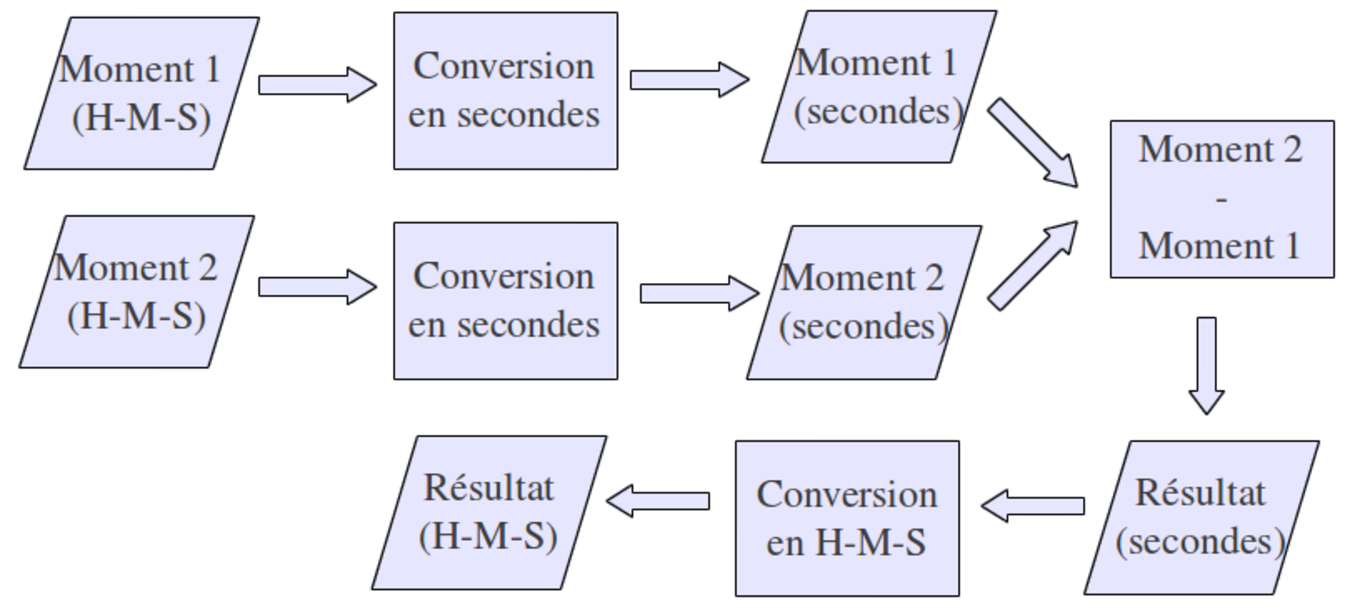
\includegraphics[width=0.8\textwidth]{image/module-conversion}
	\end{center}

\subsection*{Conversion en secondes}

	Une des sous-tâches est donc la conversion en secondes
	d'un moment exprimé en heures-minutes-secondes
	(H-M-S). Il nous faut adapter la solution trouvée pour
	l'exercice du chapitre sur les algorithmes séquentiels
	car il n'est pas question ici que les données soient
	lues ni que le résultat soit écrit ; l'interaction ne
	se fait pas avec l'utilisateur mais avec le module
	principal qui va l'utiliser.\footnote{On pourrait,
	dans notre cas précis, imaginer que le module de conversion demande les
	données à l'utilisateur mais un tel module serait
	moins souvent réutilisable.}

	La première question à se poser est donc celle des paramètres :

	\begin{liste}
	\item 
		Quelles sont les données dont a besoin l'algorithme
		pour travailler ?
	\item 
		Quels résultats fournit-il ?
	\end{liste}

	Dans notre cas, la réponse est simple :

	\begin{liste}
	\item {
		Les données sont le moment à convertir en secondes. Ce moment est
		représenté par trois entiers : les heures, les minutes et les secondes
		;}
	\item {
		Le résultat est le moment converti en secondes. Il est représenté par un
		entier.}
	\end{liste}

	Lorsque le résultat est représenté par une seule donnée, on a le choix
	entre un paramètre en sortie :

	\cadre{
	\begin{pseudo}
		\ModuleSign{HMSversSec}{H\In,M\In,S\In,secondes\Out : entiers}{}
	\end{pseudo}
	}
	
	ou une valeur de retour :

	\cadre{
	\begin{pseudo}
		\ModuleSign{HMSversSec}{H\In,M\In,S\In : entiers}{entier}
	\end{pseudo}
	}

	Dans de pareils cas, 
	on privilégie souvent la valeur de retour car cela
	facilite l'écriture lors de l'appel.

	L'algorithme s'écrit alors :

	\cadre{
	\begin{pseudo}
		\Module{HMSversSec}{H\In,M\In,S\In : entiers}{entier}
			\Decl secondes : entier \RComment A déclarer puisque ce n'est pas un paramètre
			\Let secondes \Gets  H * 3600 + M * 60 + S
			\Return secondes
		\EndModule
	\end{pseudo}
	}

	ou de manière équivalente mais plus concise :

	\cadre{
	\begin{pseudo}
		\Module{HMSversSec}{H\In,M\In,S\In : entiers}{entier}
			\Return H * 3600 + M * 60 + S
		\EndModule
	\end{pseudo}
	}

\subsection{Conversion en heures-minutes-secondes}

	À la fin de notre algorithme, il nous faudra reconvertir un résultat
	exprimé en secondes sous la forme heures-minutes-secondes. À nouveau,
	on a déjà résolu ce problème dans le chapitre sur les algorithmes
	séquentiels. Mais il faut l'adapter à
	l'usage de paramètres.

	\begin{liste}
	\item {
		Quelles sont les données ? Une seule, le moment exprimé en secondes}
	\item {
		Quels sont les résultats calculés par le module ? Ce même moment exprimé
		en heures-minutes-secondes. Trois entiers sont requis ce qui fait que
		le choix entre un paramètre en sortie et une valeur de retour ne se
		pose pas ici ; impossible d'utiliser une valeur de
		retour (qui doit être unique) ; on doit utiliser des paramètres en
		sortie.}
	\end{liste}

	Ce qui donne :

	\cadre{
	\begin{pseudo}
		\Module{secVersHMS}{secondes\In,S\Out,M\Out,S\Out : entiers}{}
			\Let H \Gets secondes DIV 3600
			\Let M \Gets secondes MOD 3600 DIV 60
			\Let S \Gets secondes MOD 60
		\EndModule
	\end{pseudo}
	}

\subsection{La solution}

	À présent, on a tout pour écrire la solution à notre problème

	\cadre{
	\begin{pseudo}
		\Module{différenceEntreHeures}{}{} \RComment Pas de paramètres !
			\Decl H1, M1, S1, H2, M2, S2 : entiers \RComment Les 2 moments à soustraire
			\Decl secondes1, secondes2 : entiers \RComment Ces 2 moments en secondes
			\Decl diffSecondes : entier \RComment La différence en secondes
			\Decl diffH, diffM, diffS : entiers \RComment La différence en H-M-S
			\Read H1, M1, S1, H2, M2, S2
			\Let secondes1 \Gets HMSversSec( H1, M1, S1 )
			\Let secondes2 \Gets HMSversSec( H2, M2, S2 )
			\Let diffSecondes \Gets secondes2 – secondes1
			\Stmt secVersHMS( diffSecondes, diffH, diffM, diffS )
			\Write diffH, diffM, diffS
		\EndModule
	\end{pseudo}
	}

	\marginicon{reflexion}
	\begin{Emphase}{Variante}
		Dans la solution ci-dessus, 
		quelle est ou quelles sont la/les variable(s) locale(s) 
		dont on pourrait se passer moyennant une réécriture de
		l'algorithme ?
	\end{Emphase}
	
\section{Blocs}

	{
	{Un bloc est l’écriture d’une portion de module
	à l’extérieur de celui-ci. C’est un simple
	}{\textit{déplacement}}{
	de lignes de codes vers un autre endroit du texte de
	l'algorithme. La raison de découper un module en blocs
	peut être le souci de clarifier un algorithme en le découpant en étapes
	bien distinctes, ou tout simplement un manque de place… Les variables
	d’un bloc ne sont donc pas des variables locales du bloc dans lequel
	elles apparaissent, mais bien des variables locales du module auquel
	appartient ce bloc. L’appel de l’exécution des instructions se trouvant
	dans un bloc est similaire à celui d’un module avec paramètres, on
	écrit simplement le nom du bloc comme s’il s’agissait d’une
	instruction.}}

	{
	Pour exemple, le module additionnerFractions (première version dans le
	chapitre 3) pourrait se découper ainsi :}

	\cadre{
	\begin{pseudo}
		\Module{additionnerFractions}{}{}
			\Stmt déclaration
			\Stmt lectureDonnées
			\Stmt calculs
			\Stmt écritureRésultat
		\EndModule
	\end{pseudo}
	}

	\cadre{
	\begin{pseudo}
	\Block{declaration}
		\Decl num1, den1, num2, den2, numRes, denRes : entiers
	\EndBlock
	\end{pseudo}
	}

	\cadre{
	\begin{pseudo}
	\Block{lectureDonnées}
		\Read num1, den1, num2, den2
	\EndBlock
	\end{pseudo}
	}

	\cadre{
	\begin{pseudo}
	\Block{calculs}
		\Let numRes \Gets num1 * den2 + num2 * den1
		\Let denRes \Gets den1 * den2
	\EndBlock
	\end{pseudo}
	}

	\cadre{
	\begin{pseudo}
	\Block{écritureRésultat}
		\Write numRes, "/", denRes \RComment la fraction n'est pas simplifiée
	\EndBlock
	\end{pseudo}
	}

	{
	{Le bloc contenant la déclaration des variables
	est aussi appelé }{\textbf{dictionnaire des
	variables}}{ du module.}}

\section{Qu'est-ce qu'un algorithme de qualité ?}

	{
	Nous voulons tous produire du code de qualité mais
	qu'est-ce que cette notion recouvre vraiment ?
	Qu'est-ce qui permet de juger de la qualité
	d'un code ? De nombreux critères existent. Citons ici,
	parmi les plus pertinents, ceux qui sont le plus liés à ce
	cours\footnote{Pour approfondir cette notion,
	l'étudiant pourra lire par exemple : Bertrand Meyer,
	«~\textit{Conception et programmation par objets : pour du logiciel de
	qualité}~», aux éditions «\textit{~interéditions~}»}. }

\subsection{La validité}

	{
	C'est l'évidence, le code doit
	réaliser les tâches pour lesquelles il a été écrit, même dans tous les
	cas particuliers imaginés. C'est là le critère
	principal et les autres ne sont là que pour aider à atteindre celui-ci
	plus facilement. Ne nous leurrons pas, ce critère est loin
	d'être facile à rencontrer. Il suffit pour
	s'en convaincre de se rappeler toutes les fois où des
	logiciels pourtant courants que nous utilisons se sont déjà arrêtés sur
	des erreurs.}

\subsection{L'extensibilité (ou évolutivité)}

	{
	Un code valide résout un problème particulier. Mais dans les situations
	réelles, le problème change régulièrement. Nous voudrons adapter le
	logiciel à de nouveaux besoins, à une modification de la législation,
	parce qu’un besoin était mal compris, ... Ces modifications peuvent
	parfois être prévues mais pas toujours.}

	{
	Le code doit être écrit de telle sorte qu'un changement
	mineur dans le problème n'implique
	qu'un changement mineur dans le code. Ce changement
	doit être évident, facile à opérer et rapide. Il ne doit pas mettre à
	mal la validité du code.}

\subsection{La réutilisabilité}

	{
	On désigne ici la capacité à réutiliser un bout de code
	d'un projet dans un autre projet. Cette réutilisation
	doit être aisée et sûre. Réutiliser du code permet
	d'utiliser du code qui a déjà été éprouvé et de gagner
	du temps que l'on pourra utiliser à améliorer le code
	que l'on doit encore écrire. La découpe en modules
	joue ici un rôle essentiel.}

\subsection{La lisibilité}

	{
	La lisibilité d'un code recouvre une notion globale et
	locale. Au niveau global, on doit facilement comprendre la structure
	générale du code afin de pouvoir aisément comprendre où se trouve le
	code qui nous intéresse. Au niveau local, on doit pouvoir comprendre
	aisément chaque bout de code.}

	{
	Au niveau du procédural (on nomme ainsi la programmation qui se
	structure à l'aide de modules), cela revient à dire
	qu'on doit rapidement voir quels sont les fonctions et
	leur rôle (niveau global) et que chaque fonction sera aisément
	compréhensible (niveau local). }
	
	{
	Est-ce que la lisibilité d'un code passe par
	l'abondance de commentaire ? Non, pas forcément. Le
	commentaire sert à expliquer ce qui n'est pas
	immédiatement clair dans le code. La première source de lisibilité
	provient donc du code lui-même. C'est pourquoi on est
	attentif à la bonne découpe en modules, au choix judicieux des noms de
	modules et de variables, ... Le respect de ces bonnes pratiques diminue
	le besoin de commentaires.}
	
\subsection{L'efficience}

	{
	Ce critère s'intéresse à la bonne utilisation des
	ressources informatiques. Est ce qu'il va tourner
	suffisamment vite, utiliser peu de mémoire ? Faut-il chercher
	systématiquement à optimiser son code ? Non ! On a souvent tendance à
	surévaluer ce critère ce qui est dommageable pour trois raisons.}

	\begin{liste}
	\item {
		Souvent, l'approche directe est suffisante. Par
		exemple, la plupart des applications sont interactives.
		C'est alors l’utilisateur qui est le plus lent, pas la
		machine qui a tout le temps d'effectuer sa tâche
		pendant que l’utilisateur réfléchit à ce qu'il doit
		taper.}
	\item {
		En général, un programme passe 80\% de son temps dans 20\% de son code.
		Chercher à optimiser chaque ligne de code est une perte de temps.}
	\item {
		Accroitre la rapidité d'un code est presque toujours en
		contradiction avec sa lisibilité. On va utiliser un algorithme moins
		connu ou des raccourcis difficiles à suivre.}
	\end{liste}

	{
	C'est pourquoi on recommande en général, face à un
	problème, d'utiliser la solution la plus courante, la
	plus claire. Une fois le programme terminé, et seulement si le besoin
	s'en fait sentir, on identifiera les portions de code
	où le programme s'attarde le plus et on cherchera à
	les optimiser.}

\section{Exercices}

\begin{Exercice}{Compréhension}
	Indiquer quels nombres sont successivement affichés lors de l’exécution
	des modules ex1, ex2, ex3 et ex4.

	\cadre{
	\begin{pseudo}
	\Module{ex1}{}{}
		\Decl x, y : entiers
		\Stmt addition( 3, 4, x )
		\Write x
		\Let x \Gets 3
		\Let y \Gets 5
		\Stmt addition( x, y, y )
		\Write y
	\EndModule

	\Empty

	\Module{addition}{a\In,b\In,c\Out: entiers}{}
		\Decl somme : entier
		\Let somme \Gets a + b
		\Let c \Gets somme
	\EndModule
	\end{pseudo}
	}

	\cadre{
	\begin{pseudo}
	\Module{ex2}{}{}
		\Decl a, b : entiers
		\Stmt addition( 3, 4, a ) \Comment voir ci-dessus
		\Write a
		\Let a \Gets 3
		\Let b \Gets 5
		\Stmt addition( b, a, b )
		\Write b
	\EndModule
	\end{pseudo}
	}

	\cadre{
	\begin{pseudo}
	\Module{ex3}{}{}
		\Decl a, b, c : entiers
		\Stmt calcul( 3, 4, c )
		\Write c
		\Let a \Gets 3
		\Let b \Gets 4
		\Let c \Gets 5
		\Stmt calcul( b, c, a )
		\Write a, b, c
	\EndModule
	\Empty
	\Module{calcul}{a\In,b\In,c\Out: entiers}{}
		\Let a \Gets 2 * a
		\Let b \Gets 3 * b
		\Let c \Gets a + b
	\EndModule
	\end{pseudo}
	}

	\cadre{
	\begin{pseudo}
	\Module{ex4}{}{}
		\Decl a, b, c : entiers
		\Let a \Gets 3
		\Let b \Gets 4
		\Let c \Gets f(b)
		\Write c
		\Stmt calcul2(a, b, c)
		\Write a, b, c
	\EndModule
	\Empty
	\Module{calcul2}{a\In,b\In,c\Out: entiers}{}
		\Let a \Gets f(a)
		\Let c \Gets 3 * b
		\Let c \Gets a + c
	\EndModule
	\Empty
	\Module{f}{a\In: entier}{entier}
		\Decl b : entier
		\Let b \Gets 2 * a + 1
		\Return b
	\EndModule
	\end{pseudo}
	}

\end{Exercice}

\begin{Exercice}{Appels de module}
	Parmi les instructions suivantes (où les variables
	\textstyleCodeInsr{a}, \textstyleCodeInsr{b} et \textstyleCodeInsr{c}
	sont des entiers), lesquelles font correctement appel au module
	d’en-tête suivant ?

	\cadre{
	\begin{pseudo}
		\ModuleSign{PGCD}{a\In,b\In: entiers}{entier}
	\end{pseudo}
	}

	\cadre{
	\begin{pseudo}
	\Stmt [1] a \Gets PGCD( 24, 32 )
	\Stmt [2] a \Gets PGCD( a, 24 )
	\Stmt [3] b \Gets 3 * PGCD( a + b, 2*c ) + 120
	\Stmt [4] PGCD( 20, 30)
	\Stmt [5] a \Gets PGCD( a, b, c )
	\Stmt [6] a \Gets PGCD( a, b ) + PGCD( a, c )
	\Stmt [7] a \Gets PGCD( a, PGCD( a, b ) )
	\Stmt [8] \K{lire} PGCD( a, b )
	\Stmt [9] \K{écrire} PGCD( a, b)
	\Stmt [10] PGCD(a, b ) \Gets c
	\end{pseudo}
	}
	
\end{Exercice}

\begin{Exercice}{Comparaison d'algorithmes}
	Soit un module testant si un nombre entier est pair.
	Comparez les différentes solutions proposées.

	\cadre{
	\begin{pseudo}
		\Module{estPair}{nb\In: entier}{booléen}
		\Decl pair : booléen
		\Let pair \Gets faux
		\If{nb MOD 2 = 0}
			\Let pair \Gets vrai
		\EndIf
		\Return pair
		\EndModule
	\end{pseudo}
	}

	\cadre{
	\begin{pseudo}
		\Module{estPair}{nb\In: entier}{booléen}
		\Decl pair : booléen
		\If{nb MOD 2 = 0}
			\Let pair \Gets vrai
		\Else
			\Let pair \Gets faux
		\EndIf
		\Return pair
		\EndModule
	\end{pseudo}
	}

	\cadre{
	\begin{pseudo}
		\Module{estPair}{nb\In: entier}{booléen}
		\Decl pair : booléen
		\Let pair \Gets nb MOD 2 = 0
		\Return pair
		\EndModule
	\end{pseudo}
	}

	\cadre{
	\begin{pseudo}
		\Module{estPair}{nb\In: entier}{booléen}
		\Return nb MOD 2 = 0
		\EndModule
	\end{pseudo}
	}

	\cadre{
	\begin{pseudo}
		\Module{estPair}{nb\In: entier}{booléen}
		\If{nb MOD 2 = 0}
			\Return vrai
		\Else
			\Return faux
		\EndIf
		\EndModule
	\end{pseudo}
	}

	\cadre{
	\begin{pseudo}
		\Module{estPair}{nb\In: entier}{booléen}
		\If{nb MOD 2 = 0}
			\Return vrai
		\EndIf
		\Return faux
		\EndModule
	\end{pseudo}
	}
	
\end{Exercice}

\begin{Exercice}{Échange de variables}
\marginicon{java}
Écrire un module \textit{swap} qui échange le contenu des deux variables
entières passées en paramètres.
\end{Exercice}

\begin{Exercice}{Valeur absolue}
Écrire un module qui retourne la valeur absolue d'un
réel reçu en paramètre.
\end{Exercice}

\begin{Exercice}{Maximum de 4 nombres}
\marginicon{java}
Écrire un module qui retourne le maximum de 4
nombres donnés en paramètres.
\end{Exercice}

\begin{Exercice}{Validité d'une date}
\marginicon{java}
Reprendre l'algorithme de validation d'une date 
développé au chapitre précédent et le rendre modulaire.
\end{Exercice}

